\documentclass{article}
\usepackage{amsmath}
\usepackage{amsfonts}
\usepackage{amssymb}
\usepackage{graphicx}
\usepackage{chngpage}
\usepackage{multicol}
\usepackage{hyperref}

\begin{document}


\title{Parallel Galaxy Simulations}

\author{Cody Garges \\ \texttt{gargec@rpi.edu} \\ \\
	James McAtamney \\ \texttt{mcataj@cs.rpi.edu} \\ \\
	Amanda Olyha \\ \texttt{olyhaa@rpi.edu} }  
\date{May 14, 2011}	
 
\maketitle


\begin{abstract}

As computing power has improved over the years, parallel applications have been developed to take advantage of the high throughputs for computationally intensive problems.  One such problem is the rendering of galaxies and their motions over time.  This paper illustrates one approach towards developing a galaxy simulator using MPI messages to share stars across multiple processors.  We examine runtimes and speedups as a result of using multiple processors to perform our work and determine what fraction of the total runtime are devoted to messaging, IO tasks, and computation.

\end{abstract}

\section{Introduction}

Galaxy simulations are a computationally intensive process.  There are billions of stars that are interacting with each other to create a stable, rotating system.  This interaction manifests in the form of gravitational forces that occur between every pair of stars. 

Galaxies come in all shapes and sizes, each with their own characteristics.  Some may have a few as ten million stars while others can have on the order of a hundred trillion stars, all orbiting a galaxy's center of mass.  In addition to stars (and their respective systems of planets, asteroids, and other objects), galaxies also contain star clusters, interstellar clouds, and dark matter.  It is the combination of all these objects that provide galactic stability for spiral galaxies, the second most abundant type of galaxy in our known universe.  These galaxies are relatively flat with large, curving arms, and generally have a spherical ``bulge'' at their center.   Since this is the model of our own Milky Way Galaxy, we will be simulating this type of galaxy for a constant number of stars.

We have used a simplified model of a galaxy due to the time and computational restrictions for the scope of this project.  We ignored the effects of small bodies such as planets since they do not have a significant contribution to the galactic forces.  We also did not include the effects of stellar gas or plasma in our preliminary models.

We found that there have been many attempts to model galaxies, as well as their collisions and creations, through the use of massively parallel systems.  Since the number of calculations that need to be performed scale on O(n$^2$), the length of simulations for very large systems can get to be quite large.  By dividing the work between many processors, the computation time can be reduced.

\section{Implementation}

\subsection{Overview}

As stated above, we modeled a spiral galaxy for a set number of stars.  The underlying architecture is built on communications through the use of MPI messages. Each processor is assigned a fraction of the galaxy to update at each timestep.  Each section contains a fraction of the stars in the galaxy as well as a fraction of the dark matter points.  In order to account for the interactions with every other mass in the galaxy, each processor's list of stars (and dark matter) are passed around to every other processor to reference in calculations.  

The main problem illustrated here is an application of the N-body problem:  we have potentially billions of stars that are interacting with each other to create a stable, rotating, system.  Each of the stars are treated as a point mass with location, velocity, and mass.  Based on the positions of these stars, we can calculate the gravitational forces between every pair of points (since it is inversely proportional to the distance between them) and then modify their respective velocities and locations.  

Since we want to obtain an accurate depiction of the real galaxies in the universe, we must also add dark matter.  There are many different theories as to how dark matter is distributed, and we will explain the model that we used for this simulation in the section concerning dark matter below.

\subsection{Data Structures}

In order to use MPI effectively, we needed a way to store our star data in a compact form that could be passed to the other processors.  To accomplish this, we have created a data structure that contains the key information about the stars in our system.  Each star is assigned an $x$, $y$, and $z$ coordinate, $x$, $y$, and $z$ components of the velocity, $x$, $y$, and $z$ components of its acceleration, as well as its mass.  

\subsection{Dark Matter}
\label{subsec:dark_matter_section}

In a Keplerian system such as this, we would expect the orbital velocity of stars to decrease by $\frac{1}{\sqrt{r}}$.  However, it has been observed that rotation curves of spiral galaxies are constant over the entire radius of the galaxy except near the center where there is an approximately linear dependence.  This constant velocity implies that the cumulative mass of the galaxy rises linearly with the radius.  This does not agree with the visible mass distributions of galaxies, so scientists have come to the conclusion that there exists mass that we cannot see, or ``dark matter''.  Dark matter is still widely unknown - we do not know how it is distributed throughout the universe or what it is actually made of.  Scientists have not been able to detect the presence of dark matter, but it is widely believed that it exists \cite{rotation-dynamics}.

For the purpose of this project, we treated dark matter as distribution of stars that remain at a fixed positions in space.  These ``stars'' are uniformly distibuted throughout the galaxy and extend radially, 50\% beyond the outer limits of the visible system.  Each of the dark matter points were given a mass of 4 solar masses since it is believed that dark matter has a greater mass than the individual stars in the galaxy.

\subsection{Initial Conditions}

In order to accurately create an initial distribution for the mass in a spiral galaxy, there are two mass distributions that we had to take into account: a spherical bulge and a thin disk.  The spherical bulge is located at the center of the galaxy, with the thin disk surrounding it \cite{rotation-dynamics}.  

\begin{figure}[Ht!]
\centering
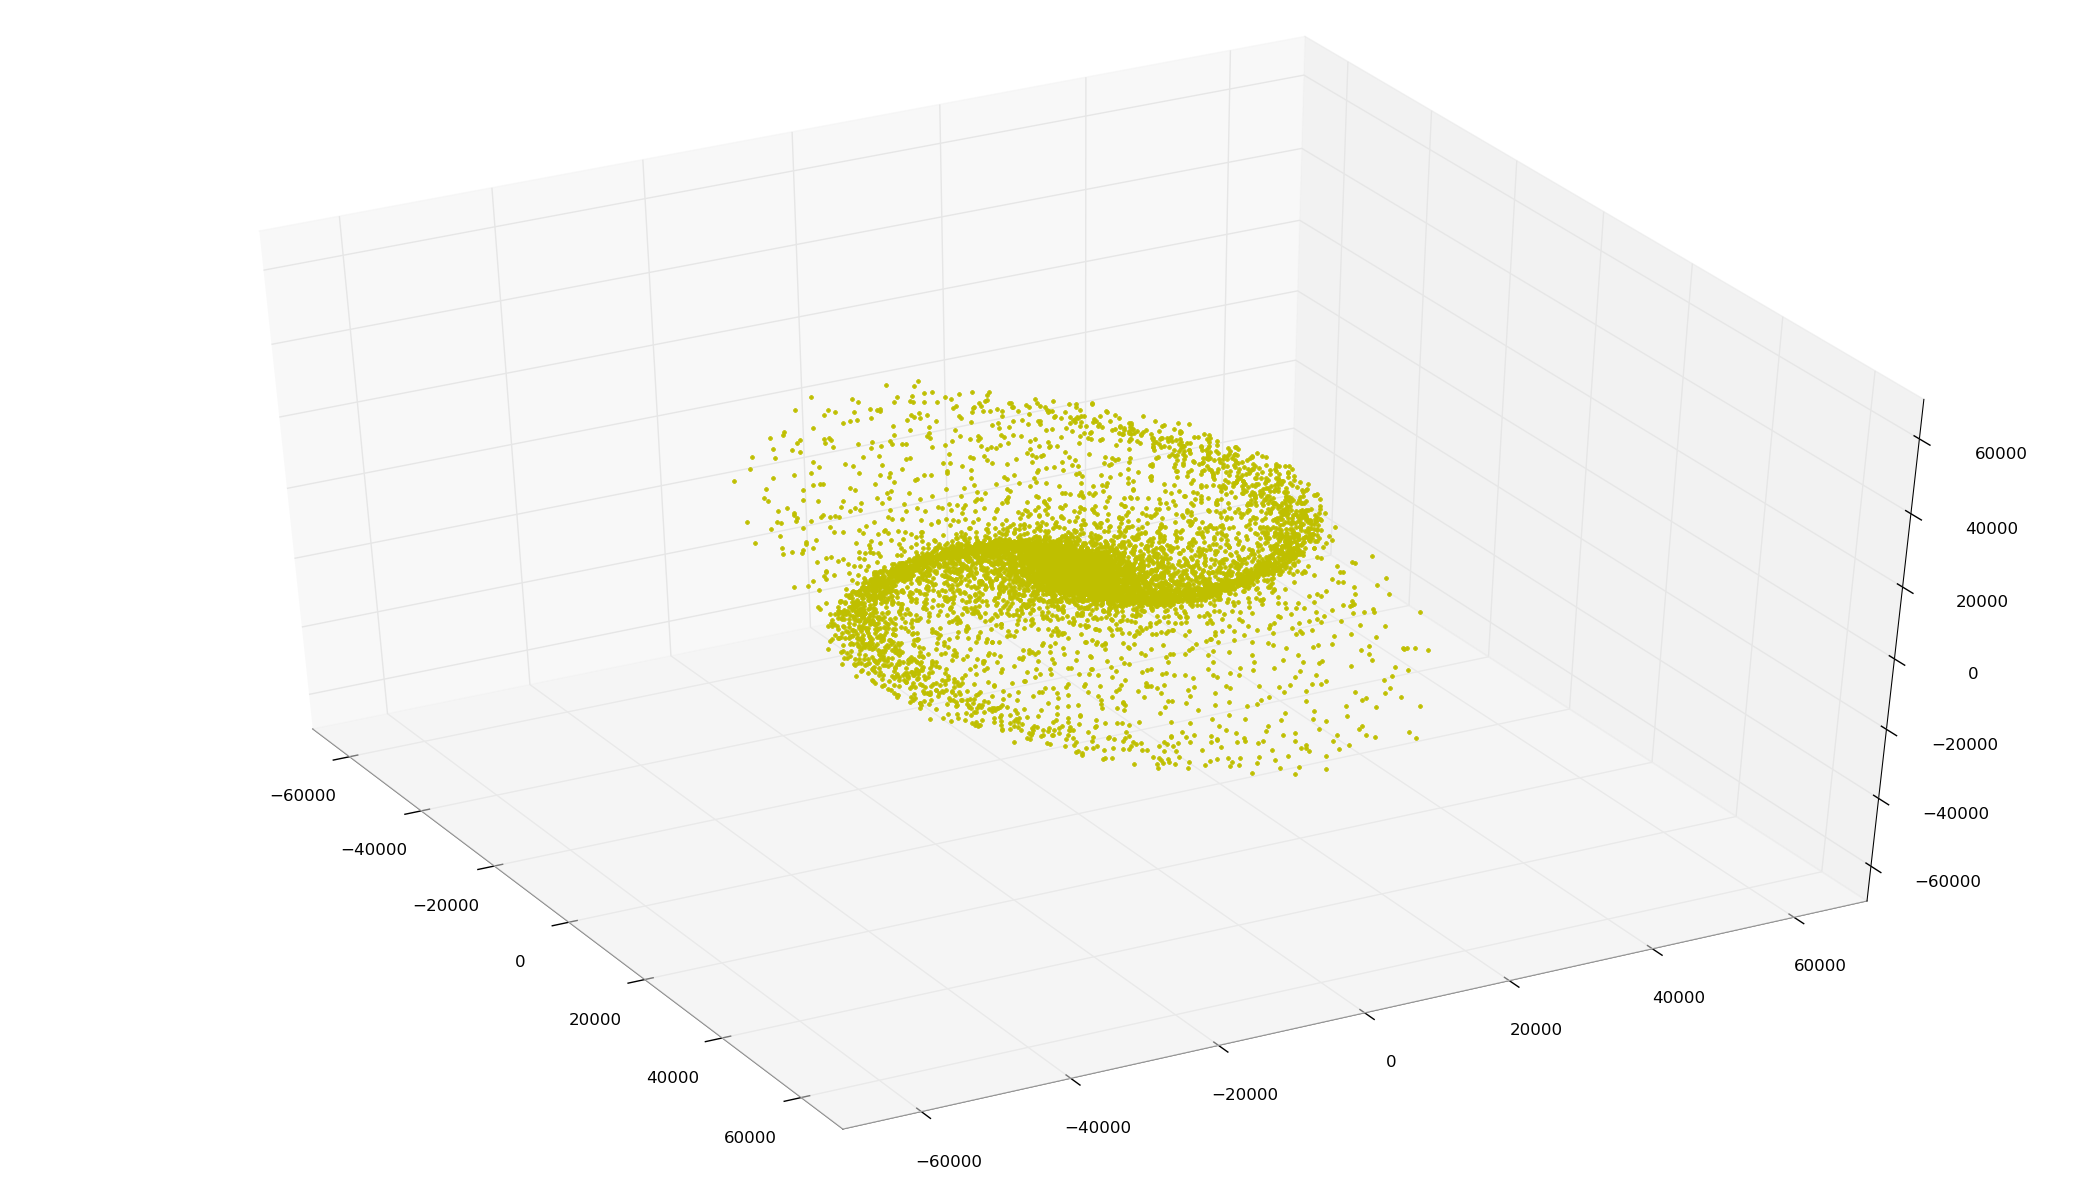
\includegraphics[width=\columnwidth]{initial-conditions.png}
\caption{The initial galaxy configuration.  It contains 12,070 stars. \label{fig:init-cond}}
\end{figure}

Since we did not want to focus on galaxy formations, we wanted to create an initial model that mirrors a real galaxy.  To generate the initial positions of the stars in the galaxy, we had to consider several properties of a spiral galaxy:
\begin{enumerate}
  \item Shape of the spiral arms and central bulge. 
  \item The density of the stars
  \item The velocity of the stars 
  \item The distribution of the dark matter. 
\end{enumerate}

In a standard spiral galaxy the arms have the shape of a logarithmic spiral. For this project we used the spiral density waves theory first developed by C. C. Lin and Frank Shu in 1964. In this model, stars have elliptical orbits and the size and rotation of these ellipses varies in a correlated way. Figure \ref{fig:spiral-arms} shows an example of this.
\begin{figure}[Ht!]
\centering
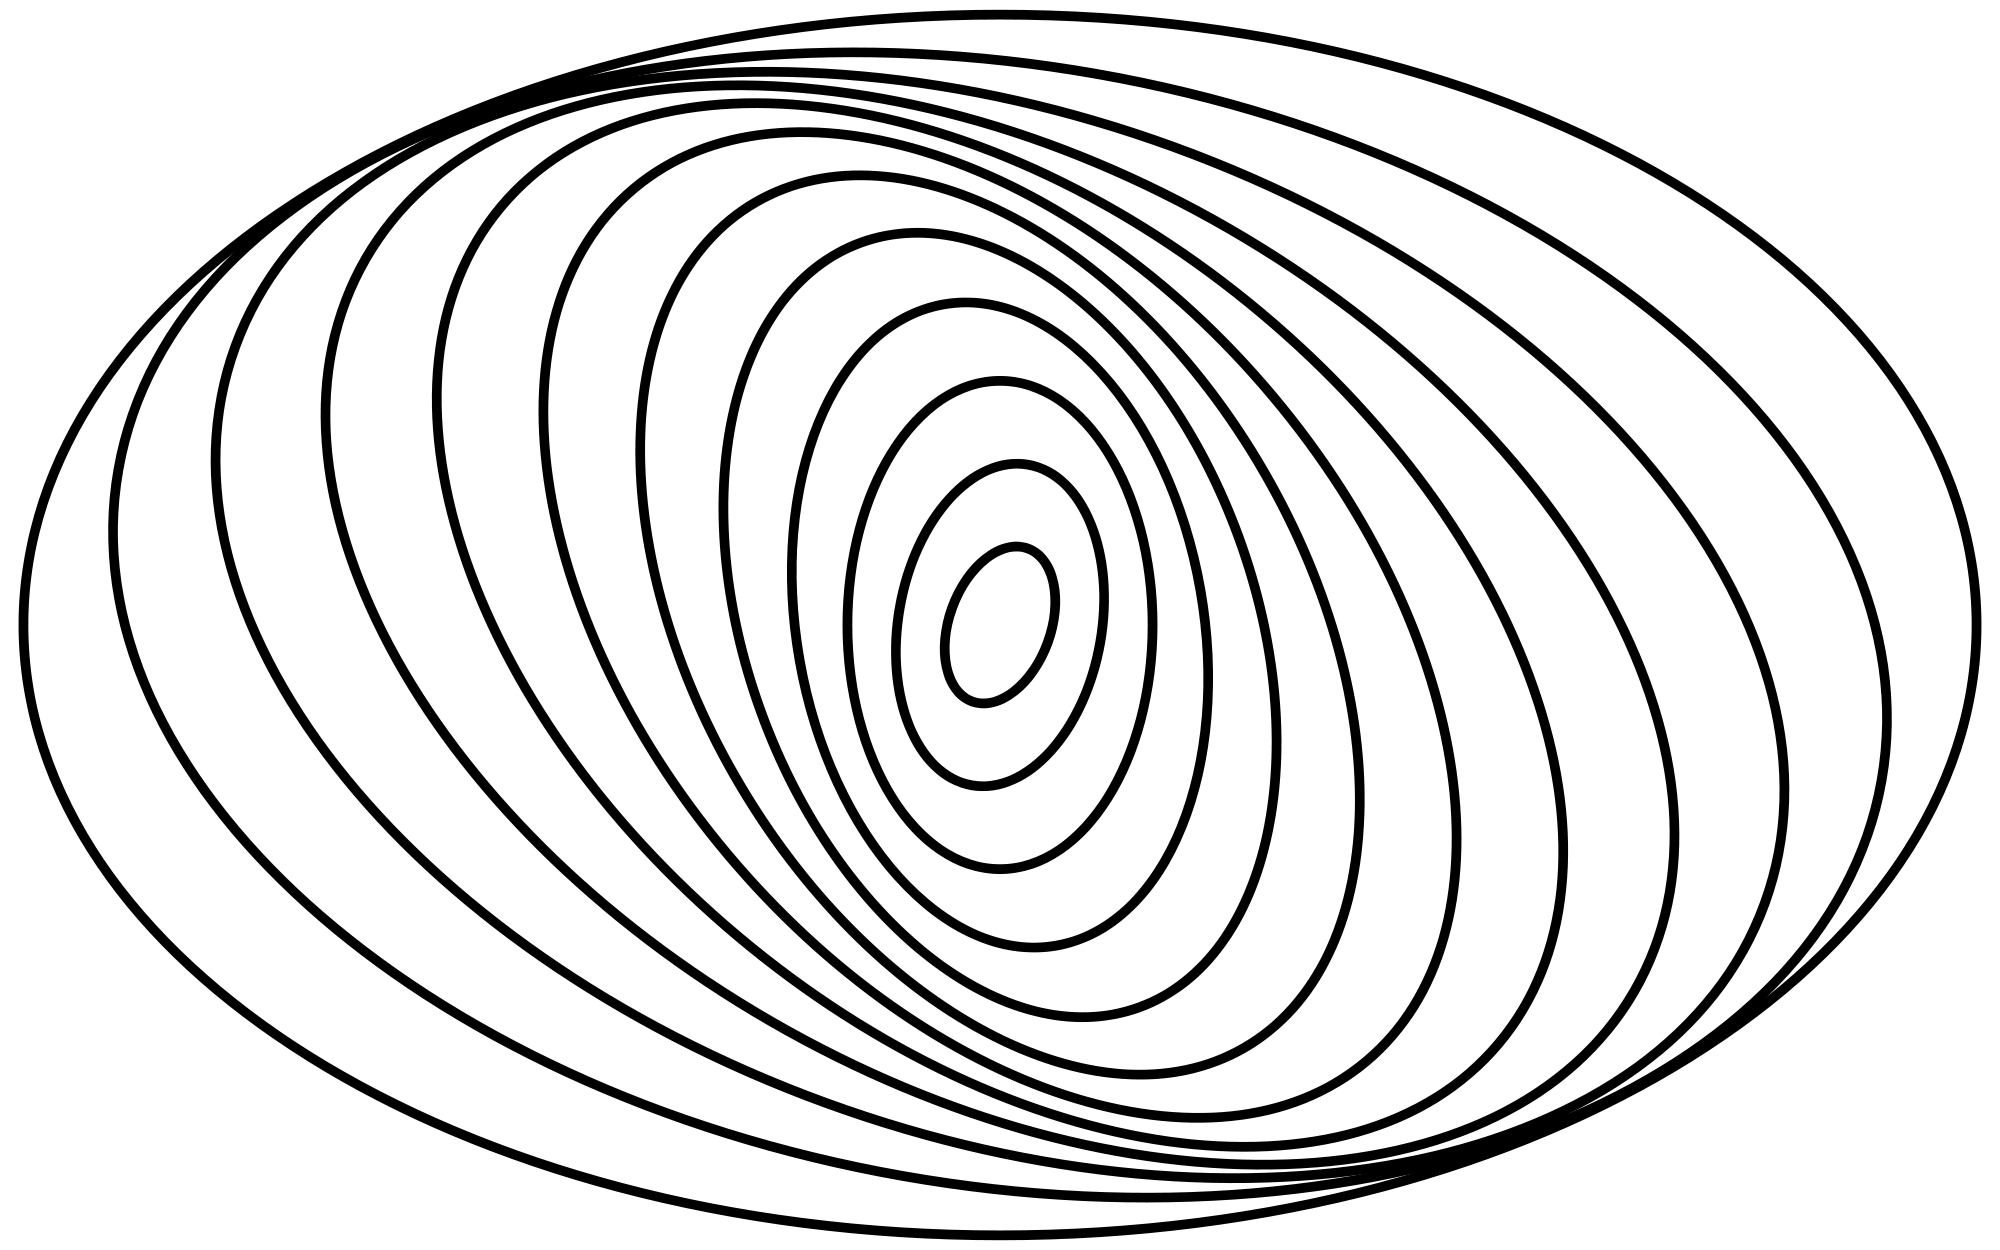
\includegraphics[width=.8\columnwidth]{spiral-arms.png}
\caption{An explanation of spiral galaxy arms.  The ellipses are stars' orbits around the galactic center.  The arms are areas of high density. \label{fig:spiral-arms}}
\end{figure}

The density of stars in a spiral galaxy is distributed according to $e^{-r}$. To generate a distribution that fit this model we created a list of ellipses, in the form of a parametric equation, that fit the model above where the density of ellipses went as $e^{-r}$. Then each ellipse was filled with the same number of stars, at a random location along the ellipse which was then slightly perturbed. The z component was then fit to a normal distribution about the x-y plane. Around the center of a normal spiral galaxy there is a central bulge. We approximated this with a constant density sphere around the origin.

\begin{figure}[Ht!]
\centering
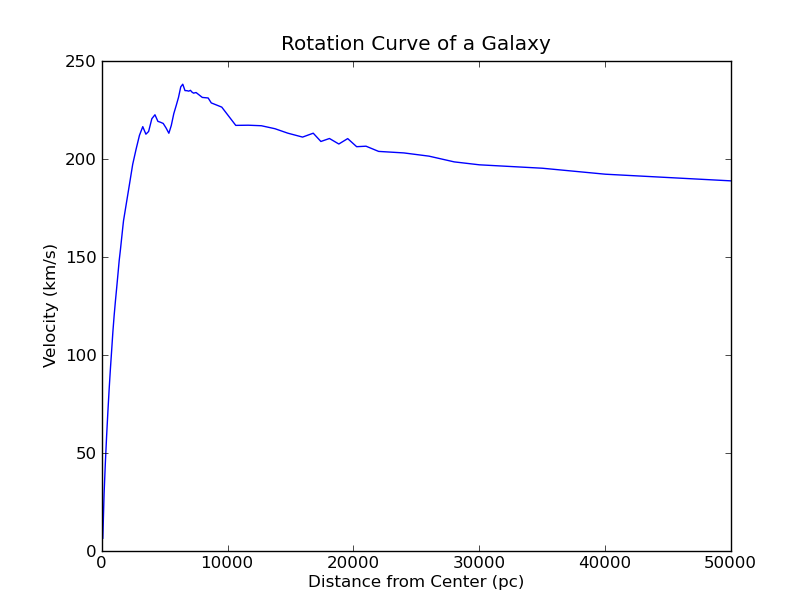
\includegraphics[width=.8\columnwidth]{rotation_curve.png}
\caption{The rotation curve we fit our initial velocities to. \cite{velocity-distributions} } 
\label{fig:vel}
\end{figure}
To find the velocities of the stars we fit the velocities to a measured rotation curve -CITE- Figure \ref{fig:vel} shows the data we fit to. The velocities in the spiral arms were then pointed along the direction of the ellipse, with a small random component. For the central bulge we had the orbits be circular around the origin but in a random plane. 

\begin{figure}[Ht!]
 \centering
 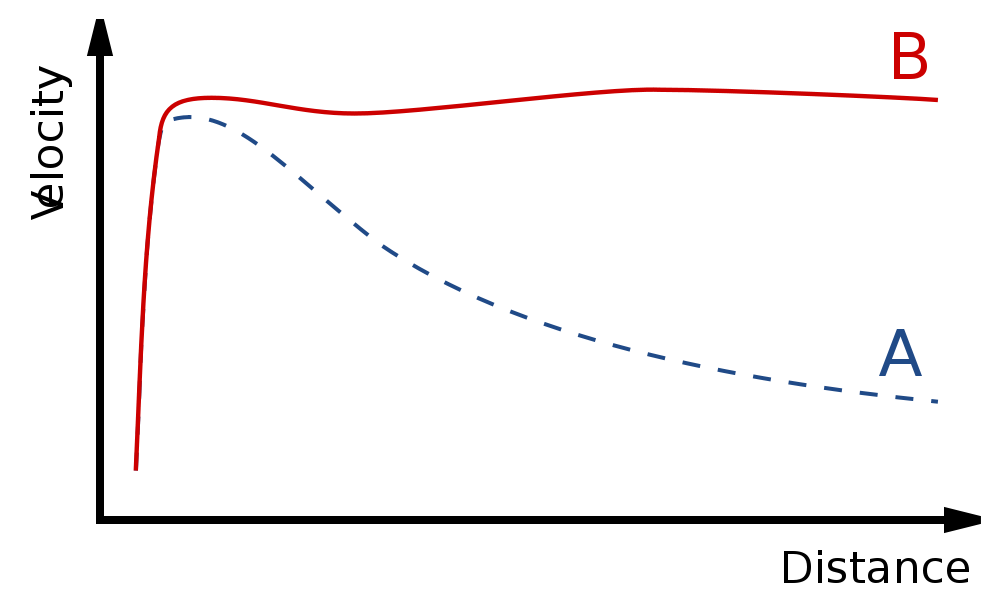
\includegraphics[width=0.5\textwidth]{./rotation.png}
  \caption{The rotation curve of the stars in a typical spiral galaxy. Curve A is the results predicted by Newtonian mechanics. Curve B is the observed results. \href{http://en.wikipedia.org/wiki/Galaxy_rotation_curve}{Source}}
 \label{fig:rot}
\end{figure}

Figure \ref{fig:rot} shows evidence for the presence of dark matter in a typical galaxy. The rotation curve of the stars in a typical spiral galaxy. Curve A is the results predicted by Newtonian mechanics. Curve B is the observed results. We also must include dark matter if we want our galaxy to be stable. We choose a spherical, constant density halo distribution of dark matter around the galaxy. Figure \ref{fig:dark} shows an example of a distribution we used. The actual distribution was dense, it was thinned out for clarity.

\begin{figure}[Ht!]
 \centering
 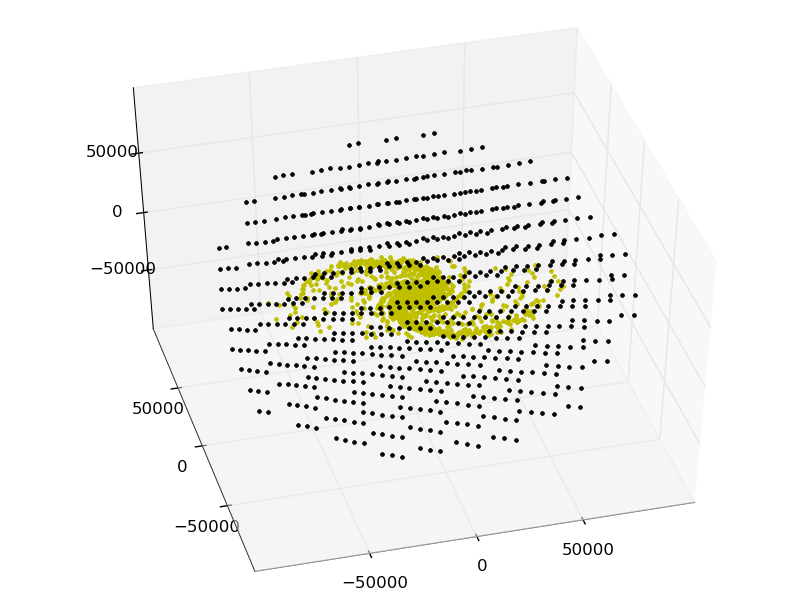
\includegraphics[width=\textwidth]{./darkmatterdist.png}
  \caption{Shows a version of the dark matter distribution we used. The actual distribution was dense, it was thinned out for clarity. } 
 \label{fig:dark}
\end{figure}

\subsection{Input and Output}
\label{subsec:io}

From the start, we decided that it would be very important to have a strict standard when dealing with input and output files.  To initialize our system, we would need to read in from a file to populate our galaxy with stars and dark matter.  Since we are aware that the simulations have the potential to run for a very long time, we needed a way to output the current state so we can use it to populate our galaxy at a later date.  In this manner, we would be able to run prolonged simulations without worrying that it would not finish within a strict time window.  

All reading and writing to files are performed in parallel using MPI file functions by all processors in the system.  Since each processor is assigned to a specific number of stars and dark matter points, it makes sense that each processor would read or write to its own personal section of the file.  By performing this task in parallel, we were able to significantly reduce the time spent reading and writing file and allow more time to be devoted to computation.

We had considered using a dedicated IO node to read and write to file, but due to the discrete and synchronous nature of this project, all nodes would need to wait for the computation to be complete since each one modifies the data throughout the compute phase.  Thus, we decided to have each processors handle its own input and output file operations.

\subsection{Algorithm}

The algorithm used to model a galaxy is based on a discrete, timestepped approach.  With each timestep, every star or dark matter point is paired up with every other star or dark matter point and the gravitational force is calculated between the two.  For a three dimensional system, this force is 

\begin{equation}
F = \frac{G \cdot m_{1} \cdot m_{2} \cdot {\bf x}}{{\bf r}^{3}}
\end{equation}

Where $G$ is the gravitational constant, $m_{1}$ and $m_{2}$ are the two masses of the stars, ${\bf x}$ is the $x$, $y$, or $z$ distance between the stars, and ${\bf r}$ is the combined distance between the two stars.  Then using Newton's second law, you can determine the acceleration caused by $m_{2}$ on $m_{1}$ using

\begin{equation}
{\bf a} = \frac{{\bf F}}{m_{1}}
\end{equation}

If you sum up every one of these small contributions from ever on of its neighbors, you can determine the total acceleration felt by the star.  As mentioned above, MPI Isends and Irecvs are used to send each processors' array of stars and dark matter points to the next processors to allow all processors to view the star's position and mass in order to calculate the needed accelerations.

Acceleration is only calculated for each of the stars - since the dark matter is not moving or changing, we have no need to calculate the acceleration for those points.

These small additions are recorded in the acceleration portion of the star data structure, as mentioned above, where they can be processed at the conclusion of all the pairwise comparisons.  At this point, we use the Verlet integration algorithm to use the accelerations to advance the stars along their trajectories according to a numerical integration scheme. Verlet's velocity formulas use the current positions, velocities, and accelerations of the star to determine its projected position and velocity at a later timestep \cite{verlet}.  These  formulas are as follows:
          
\begin{equation}
{\bf r}(t + \Delta t) = {\bf r}(t) + {\bf v}(t) \Delta t + \frac{1}{2} {\bf a}(t) \Delta t^{2}
\end{equation}         

\begin{equation}
{\bf v}(t + \Delta t) = {\bf v}(t) + {\bf a}(t) \Delta t^{2}
\end{equation}                                                                         

Where ${\bf r}$ is the position, ${\bf v}$ is the velocity, ${\bf a}$ is the acceleration, and $\Delta t$ signifies the next timestep (what we are solving for).  Once we update all the stars on the processor with this new information, we have completed one timestep.  

In order to maintain synchronization across all processors, an MPI Barrier is used to keep all processors on the same timestep.  Once all processors have passed the barrier, this process is then repeated. 

\subsection{Parameters}

For all of our tests, we started with a galaxy consisting of 12,070 stars and 17,070 dark matter points.  The timescale was chosen such that 1 timestep was equivalent to 1000 years, and we ran all of our tests for 100 timesteps to get a performance baseline.  For each run of the program, the processors initialized the galaxy by reading in values stored in the two initialization files.  The first file is a list of all the stars in the galaxy and the second file is a list of the dark matter points.  Every 10 timesteps, the processors wrote the states of all the stars to a file for later graphing.

\section{Obstacles and Difficulties}

In the course of implementing our simulation, we went through several iterations of the code as we ran into implementation difficulties.  Our first iteration was written under the assumption that the Blue Gene had global memory access (i.e. that we could have one global array that was shared between nodes as long as each node wrote to a different portion of the array) due to a misreading of the MPI specifications.  Changing the code to use standard message passing for the global array wasn't difficult, but it did take up time that could have been spent on testing.

Once we fixed the global variable issue, we ran into trouble with the CCNI Blue Gene.  Specifically, we ran into a persistent input/output error where the initial data file could be opened successfully but the processors would all idle for no discernable reason when attempting to actually read in the data.  The Blue Gene did not give a verbose error message, and there was a very long latency between submitting each run and starting each run due to the parallel computing classes taking up computation time with their final projects, which made debugging difficult; the code ran successfully on Kratos and the computer science cluster, so we abandoned the Blue Gene and used Kratos instead so as not to waste time on fixing that issue.

Finally, we ran into problems with the units used for gravitation.  Originally, to keep the numbers small, we used parsecs for distance, which resulted in a G that was too small (order of $10^{-9}$) and caused some of the stars at the very largest distances to return a gravitational force of $NaN$ after dividing this G by a distance on the order of 200,000 parsecs.  We unfortunately did not catch this error until after running our first simulation overnight for several thousand timesteps, which meant that we lost time for our subsequent runs.  After converting our units used to milliparsecs and adjusting our calculations accordingly, we resolved the $NaN$ issue.

Due to time and computational constraints, we were forced to reduce the size of our galaxy from millions or billions of stars to tens of thousands of stars, and this forced us to recalibrate our initial data to fit a sparser but just as massive galaxy.  We had several runs end with the galaxy tearing itself apart before we obtained a working dark matter and star distribution.

\section{Future Work}

Although this method for simulating galaxies is sufficient for our purposes, there are plenty of areas where algorithms and models can be improved, resulting in a more accurate and efficient method to simulate galaxy stability.

\subsection{Scaling}

If we had some more time to work on this, we would like to extend our current simulation to a larger scale galaxy with more processor counts.  It would be interesting to see where the peak performance is and if the message overheads outweigh the benefits of parallelization.

\subsection{SPH Trees}

Our current implementation of the galaxy simulation utilizes the simple parallelization of a pairwise matching scheme. While this method reduces well onto a large parallel system, it has a O(N$^2$) computation performance. The parallel nature allows optimization over the number of stars per processors in our system.  If the computations were optimized over coordinate space instead, the number of computations could be reduced further.  This would be achieved through the use of star clusters based on their relative positions in space. This method requires the subdivision of the galaxy space into sectors which could then be exported into tree structure.

Under a tree structure, each individual star would be stored in a leaf node.  The intermediate nodes can be represented as the center of mass of their children.  Siblings would be determined based on locality - stars that are in each others' immediate vicinity are more likely to be siblings than others.  In this manner, gravitational forces can be calculated using a much smaller set of points.  For stars on opposite sides of the galaxy, for example, we can approximate the gravitational force by using a multipole expansion of the intermediate nodes. This could reduce overall computations for each timestep.

A common implementation of this idea was proposed by Barnes and Hut in their SPH tree algorithm.  Since we are dealing with a collision-less system, small errors in the force for improved performance are tolerated.  These small errors arise through the use of techniques which approximate the gravitational field such as the one mentioned above.  This specific approach will scale as O(NlogN) in computational cost \cite{parallel-tree-code}.  In the original Barnes and Hut algorithm, each node has eight children, but this number can be varied as needed.  Part of a future investigation can be to evaluate different sibling configurations for efficiency and accuracy.

\subsection{Load Balancing}

In our algorithm, we did not employ any forms of load balancing.  Because we were already computing forces between every pair of stars and every processor had the same amount of stars, the load balancing was already built into our system (as shown by our relatively short amount of time spent waiting in barriers.  If we were to implement a type of SPH tree, however, we may experience some load balancing problems since some of the pair-wise computations will be combined.  The division of stars among the trees must be load balanced in order to ensure peak performance and reduce the amount of idle time for each processor \cite{parallel-treesph}. 

\subsection{Output}

For large scale simulations, it is important that you can keep track of the current state of the system in the case of error recovery, or in our case, limited time on massively parallel machines.  Because of this, we developed an output convention (see Section \ref{subsec:io}) that keeps track of every star's position, velocity and mass.  For very large systems, storing all of this information becomes a problem.  In the simulations that we ran (on the order of 12,000 stars) each output file is 1.5MB.  If we wanted to simulate our own Milky Way Galaxy (which is on the order of 400 billion stars), a single output file would be close to 50 terabytes.  This amount of data is can be impractical, especially if you are outputting the state of the galaxy at regular intervals.  If we were to increase our galaxy size, this may be something that we would want to improve.  To do this, it may be possible to compress or group the stars into clusters (perhaps our intermediate nodes) that can be extrapolated to their original distribution. This way, we can still have all of our information, but store it on less hard drive space.  

\subsection{Different Models of Dark Matter}

As mentioned in Section \ref{subsec:dark_matter_section}, dark matter is a great unknown in the area of astrophysics.  There are many theories as to what dark matter is and how it is distributed in our universe.  We used a discretized model of dark matter, but a more accurate model may be a continuous ``sheet'' that blankets a galaxy.  In addition, the density is most likely nonuniform, but more dense near the middle ranges from the galactic center \cite{dark-halo}.  Experimentally, it has been found that dark matter actually grows throughout time, so for an accurate model, this should also be observed.  If we are able to base growth and movement of dark matter on what has been observed, an even clearer picture of the universe can be uncovered.

\subsection{Other Considerations}

In addition to gravitational forces, electromagnetic forces from plasma play an important role in young galaxies.  In an older galaxy such as the one we modeled here, plasma is only a small fraction of the total mass of the galaxy and can be ignored.  If we were to extend our simulation to encompass galaxy formation, we would need a way to account for these effects.  The first step would be to create a data structure or model to account for the plasma gas.  Once we have a way to model this, we would then need add a function to calculate magnetic forces similar to our existing function that calculates gravitational forces.  This can then be easily incorporated to determine the movement and velocities of our stars.

\section{Conclusions}

This project gave us a good insight into the world of astrophysics simulations.  Although our implementation is a very small scale model of the real galaxies present in our universe, the main concepts remain the same.  While we were not able to simulate the galaxy as long as we wanted or as efficiently as we wanted due to time constraints, and while we ran into plenty of difficulties in the implementation, we still consider this a valuable learning experience despite the difficulties.

\begin{thebibliography}{99}

\bibitem{parallel-tree-code}
	Dubinski, John.
	``A Parallel Tree Code'',
	\emph{University of California, Santa Cruz}.
	March 1996.
	
\bibitem{verlet}
	Ercolessi, Furio.
	``The Verlet Algorithm'',
	http://www.fisica.uniud.it/\textasciitilde ercolessi/md/\- md/node21.html,
	September 1997.
	
\bibitem{parallel-treesph}
	Lia, Cesario and Giovanni Carraro.
	``A parallel TreeSPH code for galaxy formation'',
	\emph{University of Padova, Italy}.
	April 1999.
	
\bibitem{spiral-arms}
	Lin, C.C., F.H. Shu.
	``On the spiral structure of disk galaxies'',
	\emph{The Astrophysical Journal}.
	Volume 140.
	August 1964.
  
\bibitem{rotation-dynamics}
  Marmet, Louis.
  ``Rotation Dynamics of a Galaxy with a Double Mass Distribution'',
  November 2007.
  
\bibitem{velocity-distributions}
	McGaugh, Stacy.
	``The Rotation Curves of Low Surface Brightness Galaxies''.
	\emph{National Science Foundation},
	http://www.astro.umd.edu/\textasciitilde ssm/data.
  
\bibitem{universe_on_supercomputer}
  White, Simon D.M., and Volker Springel.
  ``Fitting the Universe on a Supercomputer'',
  \emph{Computing in Science \& Engineering}.
  March 1999.
  
\bibitem{dark-halo}
	Zhao, D.H., et al.
	``Universal Models for the Mass Accretion Histories and Concetrations of Dark Matter Halos'',
	\emph{The Astrophysical Journal},
	Decemeber 2009.
	  

\end{thebibliography}

\end{document}